\documentclass[runningheads,a4paper]{llncs}
\usepackage{amssymb}
\setcounter{tocdepth}{3}
\newcommand{\keywords}[1]{\par\addvspace\baselineskip
\noindent\keywordname\enspace\ignorespaces#1}

\usepackage[hide]{ed}
\usepackage[utf8]{inputenc}
\usepackage{lststex}
\usepackage{paralist}
\lstset{basicstyle=\sf,columns=fullflexible,showstringspaces=false}
% \usepackage{url}
% \usepackage{wrapfig}
\usepackage{tikz,standalone}
\usetikzlibrary{backgrounds,shapes,fit,shadows}
\makeatletter../../WP6/tikz/pgflibrarytikzmmt.code.tex\makeatother
\usepackage{wrapfig}
\usepackage{xspace}
\usepackage{hyperref}
\usepackage{stex-logo}
\usepackage{../CICM2016/odksystems}
\usepackage[style=alphabetic,backend=bibtex]{biblatex}
\addbibresource{kwarc.bib}% do not change
\addbibresource{../CICM2016/rest.bib}% add bibs here!
\renewbibmacro*{event+venue+date}{}
\renewbibmacro*{doi+eprint+url}{%
  \iftoggle{bbx:doi}
    {\printfield{doi}\iffieldundef{doi}{}{\clearfield{url}}}
    {}%
  \newunit\newblock
  \iftoggle{bbx:eprint}
    {\usebibmacro{eprint}}
    {}%
  \newunit\newblock
  \iftoggle{bbx:url}
    {\usebibmacro{url+urldate}}
    {}}
\title{Interoperability in the \ODK Project:\\
The Math-in-the-Middle Approach}
\author{Paul-Olivier Dehaye\inst{3} Michael Kohlhase\inst{2} Alexander
  Konovalov\inst{4} Samuel Lelièvre\inst{1} Markus
  Pfeiffer\inst{4} Nicolas M. Thiéry\inst{1}}
\institute{
  Universit\'e Paris-Sud\and
Jacobs University \and 
  University of Z\"urich \and
  University of St~Andrews
}
\providecommand\ifprefchar[2]{}% fix biblatex
\newcommand\defemph[1]{\textbf{#1}}
%\renewcommand{\ednote}[1]{}

\begin{document}
\maketitle

\ednote{NT: fix the over-capitalization of section titles (matter of taste)}
\ednote{NT: explain how this relates to other efforts in the same direction, in particular OpenMath}
\ednote{R3: (WP6 in the abstract) seems slightly too specific for outside world to care about}
\ednote{R3: "This information architecture..." - Are you sure that Math-in-the-Middle is an information architecture?}

\section{Introduction}

\ednote{NT: wondering if the next three paragraph would not fit better
  in the odk section; the reader more interested by the MitM part may
  be put off by this long discussion}

From their earliest days, computers have been used in pure mathematics, either to make
tables, to prove theorems (famously the four colour theorem) or, as with the astronomer's
telescope, to explore new theories. Computer-aided experiments, and the use of databases
relying on computer calculations such as the Small Groups Library in GAP, the Modular
Atlas in group and representation theory, or the $L$-functions and Modular Forms Database (\LMFDB, see later), are part of the standard
toolbox of the pure mathematician, and certain areas of mathematics completely depend on
it. Computers are also increasingly used to support collaborative work and education.

The last decades witnessed the emergence of a wide ecosystem of open-source tools to
support research in pure mathematics. This ranges from specialized to general purpose
computational tools such as \GAP, \PariGP, \Linbox, \MPIR, \Sage, or \Singular, via online
databases like the \LMFDB and does not count online services like Wikipedia, \Arxiv, or
MathOverflow. A great opportunity is the rapid emergence of key technologies, and in
particular the \Jupyter (previously \IPython) platform for interactive and exploratory
computing which targets all areas of science.  \ednote{R3: "does not count online services
  like Wikipedia" - why not, specifically?}

This has proven the viability and power of collaborative open-source development models,
by users and for users, even for delivering general purpose systems targeting a large
public (researchers, teachers, engineers, amateurs, \ldots). Yet we are still missing
\emph{Virtual Research Environments} (VRE), that combine these tools and present a uniform
work environment to the user, and enable groups of researchers, typically widely
dispersed, to work collaboratively on a per project basis. This is exactly where the \ODK
project kicks in.  \ednote{R3: "These can be subsumed by the goal of Virtual Research
  Environments" - I'm not sure I totally believe this claim, vis a vis the
  long-term/large-scale outreach items.}

\section{Integrating Mathematical Software Systems via the Math-in-the-Middle Approach}\label{sec:mitm}

% Mathematics has a rich notion of data: it can be either numeric or symbolic data;
% knowledge about mathematical objects given as statements (definitions, theorems or
% proofs); or software that computes with these mathematical objects. All this data is
% really a common resource, and should be maintained as such

\ednote{NT: I don't know how much highlight we want to put on VREs or
  ODK here. Of course, we are doing our experimentations with the ODK
  components. But it's about large scale integration of math software
  components in general, not necessarily just in the context of VREs.}

To achieve the goal of assembling the ecosystem of mathematical software systems in the
\ODK project into a coherent mathematical VRE, we have to make the systems interoperable at
a mathematical level. In particular, we have to establish a common meaning space that
allows to share computation, visualization of the mathematical concepts, objects, and
models (COMs) between the respective systems. Building on this we can build a VRE with
classical techniques for integrated development environments (IDE).
\ednote{R1: What is the effort involved in creating the interface theories? Can 
this be somehow characterized in general, or perhaps (e.g., using time as a 
measure of effort) by illustration based on the example included in the paper? 
Does the approach require that every piece of the source system be translated 
individually and statically inserted into the wrapper? If a new component is 
added to the source (an update), does a corresponding new component need to 
be added manually to the interface, or does the interface somehow provide a 
mechanism for automatic updates to incorporate new translations from an 
existing source? (In other words, is the wrapper in fact a complete re-implementation 
of the source functionality in the MitM language, or is a run-time translator 
that runs between the source and the mediator?)}
\ednote{R3: "a common meaning space that allows to share computation" - just one example 
of nonstandard grammar in this paper}
\ednote{R3: "Building on this we can build a VRE with classical techniques for integrated 
development environments" - Perhaps you could add a reference to a comparison case or two 
that would back up this claim.}

\subsection{A Common Meaning Space for Interoperability}

Concretely, the problem is that the software systems in \ODK have different coverage, and
where these overlap representations of and functionalities for the COMs involved differ.
This starts with simple naming issues (\emph{e.g.}\ elliptic curves are named
\lstinline|ec| in the \LMFDB, and as \lstinline|EllipticCurve| in \Sage), persists through
the underlying data structures (permutations are represented as products of cycles in
\GAP, in list form in \Sage, and in differing representations in the various tables of the
\LMFDB), and becomes virulent at the level of algorithms, their parameters, and domains of
applicability.

To obtain a common meaning space for a VRE, we have the three well-known approaches in
Figure~\ref{fig:interop}.
\begin{figure}[ht]\centering
  \begin{tabular}{|c|c|c|}\hline
    peer to peer & open standard & industry standard\\\hline
    \documentclass{standalone}
\usepackage{tikz}
\begin{document}
    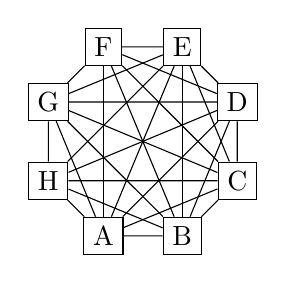
\begin{tikzpicture}
      \node[draw] (a) at (0,.3) {A};
      \node[draw] (b) at (1,.3) {B};
      \node[draw] (c) at (1.7,1) {C};
      \node[draw] (d) at (1.7,2) {D};
      \node[draw] (e) at (1,2.7) {E};
      \node[draw] (f) at (0,2.7) {F};
      \node[draw] (g) at (-.7,2) {G};
      \node[draw] (h) at (-.7,1) {H};
      \draw (a) -- (b) -- (c) -- (d) -- (e) -- (f) -- (g) -- (h) -- (a);
      \draw (a) -- (c) -- (h) -- (d) -- (g) -- (e);
      \draw (b) -- (h);
      \draw (b) -- (f);
      \draw (b) -- (d);
      \draw (b) -- (g);
      \draw (b) -- (e);
      \draw (h) -- (e);
      \draw (d) -- (f);
      \draw (g) -- (c);
      \draw (a) -- (d);
      \draw (a) -- (e);
      \draw (a) -- (f);
      \draw (a) -- (g);
      \draw (e) -- (c);
      \draw (c) -- (f);
    \end{tikzpicture}
\end{document}
%%% Local Variables: 
%%% mode: latex
%%% TeX-master: t
%%% End: 
 & \documentclass{standalone}
\usepackage{tikz}
\begin{document}
    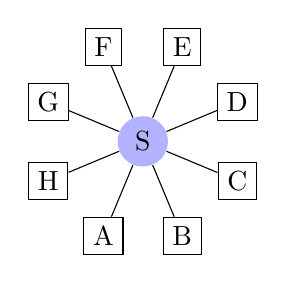
\begin{tikzpicture}
      \node[draw] (a) at (0,.3) {A};
      \node[draw] (b) at (1,.3) {B};
      \node[draw] (c) at (1.7,1) {C};
      \node[draw] (d) at (1.7,2) {D};
      \node[draw] (e) at (1,2.7) {E};
      \node[draw] (f) at (0,2.7) {F};
      \node[draw] (g) at (-.7,2) {G};
      \node[draw] (h) at (-.7,1) {H};
      \node[circle,fill=blue!30] (m) at (.5,1.5) {S};
      \draw (m) -- (a);
      \draw (m) -- (b);
      \draw (m) -- (c);
      \draw (m) -- (d);
      \draw (m) -- (e);
      \draw (m) -- (f);
      \draw (m) -- (g);
      \draw (m) -- (h);
    \end{tikzpicture}
\end{document}
%%% Local Variables: 
%%% mode: latex
%%% TeX-master: t
%%% End: 
 & \documentclass{standalone}
\usepackage{tikz}
\begin{document}
    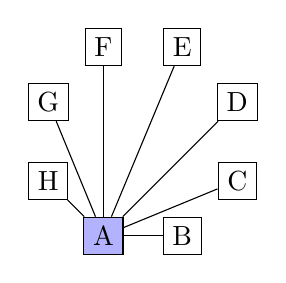
\begin{tikzpicture}
      \node[draw,fill=blue!30] (a) at (0,.3) {A};
      \node[draw] (b) at (1,.3) {B};
      \node[draw] (c) at (1.7,1) {C};
      \node[draw] (d) at (1.7,2) {D};
      \node[draw] (e) at (1,2.7) {E};
      \node[draw] (f) at (0,2.7) {F};
      \node[draw] (g) at (-.7,2) {G};
      \node[draw] (h) at (-.7,1) {H};
      \draw (a) -- (b);
      \draw (a) -- (c);
      \draw (a) -- (d);
      \draw (a) -- (e);
      \draw (a) -- (f);
      \draw (a) -- (g);
      \draw (a) -- (h);
    \end{tikzpicture}
\end{document}
%%% Local Variables: 
%%% mode: latex
%%% TeX-master: t
%%% End: 
\\\hline
    $n^2/2$  translations & $2n$ translations & $2n-2$ translations \\
    symmetric & symmetric & asymmetric\\\hline
  \end{tabular}
  \caption{Approaches for many-systems interoperability}\label{fig:interop}
\end{figure}

The first does not scale to a project with about a dozen systems, for the third there is
no obvious contender in the \ODK ecosystem. Fortunately, we already have a ``standard'' for
expressing the meaning of COMs -- \defemph{mathematical vernacular}: the language of
mathematical communication, and in fact all the COMs supported in the \ODK VRE are documented
in mathematical vernacular in journal articles, manuals, etc.
\ednote{R3: "mathematical vernacular" - This is sometimes used in a specific formal way, you 
might need to distinguish your usage from that.  (I.e. *which* mathematical vernacular are you 
referring to.)}

The obvious problem is that mathematical vernacular is too 
\begin{inparaenum}[\em i\rm)]
\item \emph{ambiguous}: we need a human to understand structure, words, and symbols
\item \emph{redundant}: every paper introduces slightly different notions. 
\end{inparaenum}

Therefore we explore an approach, where we \defemph{flexiformalize} (i.e. partially formalize;
see~\cite{Kohlhase:tffm13}) mathematical vernacular to obtain a flexiformal ontology of
mathematics that can serve as an open communication vocabulary. We call the approach the
\defemph{Math-in-the-Middle} (MitM) Strategy for integration and the ontology the \defemph{MitM
ontology}.

\begin{wrapfigure}r{4cm}\vspace*{-1.5em}
  \documentclass{standalone}
\usepackage[mh]{mikoslides}
% this file defines root path local repository
\defpath{MathHub}{/Users/kohlhase/localmh/MathHub}
\mhcurrentrepos{MiKoMH/talks}
\libinput{WApersons}
% we also set the base URI for the LaTeXML transformation
\baseURI[\MathHub{}]{https://mathhub.info/MiKoMH/talks}

\libinput{preamble}
\begin{document}
    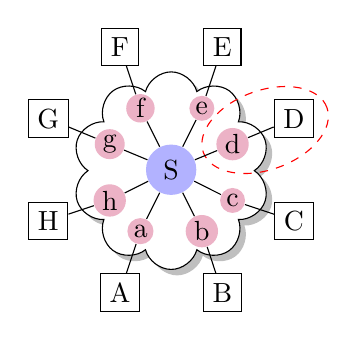
\begin{tikzpicture}[scale=1.3]
      \tikzstyle{withshadow}=[draw,drop shadow={opacity=.5},fill=white]
      \tikzstyle{system}=[draw]
      \tikzstyle{standard}=[circle,fill=blue!30]
      \tikzstyle{interface}=[circle,fill=purple!30,inner sep = 1pt,]
      \node[system] (a) at (0,.3) {A};
      \node[system] (b) at (1,.3) {B};
      \node[system] (c) at (1.7,1) {C};
      \node[system] (d) at (1.7,2) {D};
      \node[system] (e) at (1,2.7) {E};
      \node[system] (f) at (0,2.7) {F};
      \node[system] (g) at (-.7,2) {G};
      \node[system] (h) at (-.7,1) {H};
      \node[standard] (m) at (.5,1.5) {S};
      \node[interface] (ia) at (0.2,.9) {a};
      \node[interface] (ib) at (.8,.9) {b};
      \node[interface] (ic) at (1.1,1.2) {c};
      \node[interface] (id) at (1.1,1.75) {d};
      \node[interface] (ie) at (.8,2.1) {e};
      \node[interface] (if) at (0.2,2.1) {f};
      \node[interface] (ig) at (-.1,1.75) {g};
      \node[interface] (ih) at (-.1,1.2) {h};
      \draw (m) -- (ia) -- (a);
      \draw (m) -- (ib) -- (b);
      \draw (m) -- (ic) -- (c);
      \draw (m) -- (id) -- (d);
      \draw (m) -- (ie) -- (e);
      \draw (m) -- (if) -- (f);
      \draw (m) -- (ig) -- (g);
      \draw (m) -- (ih) -- (h);
      \begin{pgfonlayer}{background}
        \node[draw,cloud,fit=(ia) (ib) (ic) (id) (ie) (if) (ig) (ih),
                   inner sep=-7pt,withshadow] (st) {};
        \node[fit=(d) (id),ellipse,inner sep=-1pt,rotate=20,draw,dashed,red] (sys) {};
      \end{pgfonlayer}
      \end{tikzpicture}
\end{document}
%%% Local Variables: 
%%% mode: latex
%%% TeX-master: t
%%% End: 
\vspace*{-.5em}
  \caption{Interface theories}\label{fig:interface-theories}\vspace*{-1em}
\end{wrapfigure}
Before we go into any detail about how this ontology looks and how it induces a uniform
meaning space, we have to address another problem: the descriptions in the MitM ontology
must at the same time be system-near to make interfacing easy for systems, and serve as
an interoperability standard -- \emph{i.e.}\ be general and stable. If we have an ontology system
that allows modular/structured ontologies, we can solve this apparent dilemma by
introducing \defemph{interface theories}~\cite{KohRabSac:fvip11}, \emph{i.e.}\ ontology modules
(the light purple circles in Figure~\ref{fig:interface-theories}) that are at the same
time system-specific in their description of COMs -- near the actual representation of the
system and part of the greater MitM ontology (depicted by the cloud in
Figure~\ref{fig:interface-theories}) as they are connected to the core MitM ontology (the
blue circle) by views we call \defemph{interviews} (see below). The MitM approach
stipulates that interface theories and interviews are maintained and released together with
the respective systems, whereas the core MitM ontology represents the mathematical scope
of the VRE and is maintained with it. In fact in many ways, the core MitM ontology is the
conceptual essence of the mathematical VRE.
\ednote{R1: The choice of the term "interviews" is unfortunate because the common meaning 
of that word is not based on "inter-views". If a better term cannot be found, perhaps 
the inclusion of a hyphen would help a reader by reducing the inclination to misunderstand the term.}
\ednote{R3: "Before we go into any detail about how this ontology looks" - I think before going 
further you should add a few more details about what the process of flexiformalization is, 
or at least pointing out that there will be an example presented in Section 4}
\ednote{R3: "must at the same time be system-near" - at the same time as...?}
\ednote{R3: "in many ways, the core MitM ontology is the conceptual essence of the 
mathematical VRE." - interesting.}

\subsection{Realizing and Utilizing a MitM Ontology}

\begin{figure}[ht]\centering
  \documentclass{standalone}
\usepackage[mh]{mikoslides}
% this file defines root path local repository
\defpath{MathHub}{/Users/kohlhase/localmh/MathHub}
\mhcurrentrepos{MiKoMH/talks}
\libinput{WApersons}
% we also set the base URI for the LaTeXML transformation
\baseURI[\MathHub{}]{https://mathhub.info/MiKoMH/talks}

\usetikzlibrary{backgrounds,shapes,fit,shadows,mmt}
\begin{document}
\begin{tikzpicture}[xscale=2.6,yscale=.9]
  \tikzstyle{withshadow}=[draw,drop shadow={opacity=.5},fill=white]
   \tikzstyle{database} = [cylinder,cylinder uses custom fill,
      cylinder body fill=yellow!50,cylinder end fill=yellow!50,
      shape border rotate=90,
      aspect=0.25,draw]
   \tikzstyle{human} = [red,dashed,thick]
   \tikzstyle{machine} = [green,dashed,thick]

\node[thy]  (mf) at (.2,5.3) {MathF};
\node[thy,dashed]  (compf) at (0,6) {CompF};
\node[thy,dashed]  (pf) at (-.9,5.5) {PyF};
\node[thy,dashed]  (cf) at (1,5.5) {C\textsuperscript{++}F};
\node[thy,dashed]  (sf) at (-0.9,4.6) {SAGE};
\node[thy,dashed]  (gf) at (1,4.6) {GAP};

\draw[include] (compf) -- (pf);
\draw[includeleft] (compf) -- (cf);
\draw[include] (pf) -- (sf);
\draw[includeleft] (cf) -- (gf);

\node[thy] (kec) at (0,3) {EC};
\node[thy,minimum height=.4cm] (kl) at (0,4) {\ldots};

\node[thy] (sec) at (-1,2) {SEC};
\node[thy,minimum height=.4cm] (sl) at (-1,3) {\ldots};

\node[thy] (gec) at (1,2) {GEC};
\node[thy,minimum height=.4cm] (gl) at (1,3) {\ldots};

\node[thy] (lec) at (-.3,1.2) {LEC};
\node[thy,minimum height=.4cm] (ll) at (.3,1.2) {\ldots};

\node (sc) at (-2,4) {SAGE};
\node[draw] (salg) at (-2,3.35) {Algo};
\node[database,dashed] (sdb) at (-2,2.4) {DB?};
\node[draw] (skr) at (-2,1.7) {KR};
\node[draw,machine] (sac) at (-2,1) {AbsClass};

\node (gc) at (2,4) {GAP};
\node[draw] (galg) at (2,3.35) {Algo};
\node[database,dashed] (gdb) at (2,2.4) {DB?};
\node[draw] (gkr) at (2,1.7) {KR};
\node[draw,machine] (gac) at (2,1) {AbsClass};

\node (lmfdb) at (0,0) {LMFDB};
\node[database] (ldb) at (1,-.4) {Mongo};
\node[draw] (knowls) at (-1,-.4) {Knowls};
\node[draw,machine] (lac) at (0,-.5) {AbsClass};

  \begin{pgfonlayer}{background}
    \node[draw,cloud,fit=(sec) (sl),aspect=.4,inner sep=-3pt,withshadow,purple!30] (st) {};
    \node[draw,cloud,fit=(gec) (gl),aspect=.4,inner sep=-4pt,withshadow,purple!30] (gt) {};
    \node[draw,cloud,fit=(kec) (kl),aspect=.4,inner sep=0pt,withshadow,blue!30] (kt) {};
    \node[draw,cloud,fit=(lec) (ll),aspect=2.5,inner sep=-7pt,withshadow,purple!30] (lt) {};
  \end{pgfonlayer}

\begin{pgfonlayer}{background}
  \node[draw,withshadow,fit=(sc) (skr) (sac) (sdb),inner sep=1pt] {};
  \node[draw,withshadow,fit=(gc) (gkr) (gac) (gdb),inner sep=1pt] {};
  \node[draw,withshadow,fit=(lmfdb) (lac) (ldb) (knowls),inner sep=1pt] {};
\end{pgfonlayer}

\draw[view] (kec) -- (sec);
\draw[view] (kec) -- (gec);
\draw[view] (kec) -- (lec);
\draw[include] (kec) -- (kl);
\draw[include] (gec) -- (gl);
\draw[include] (sec) -- (sl);
\draw[include] (lec) -- (ll);
\draw[view] (kl) -- (sl);
\draw[view] (kl) -- (gl);
\draw[view] (kl) to[bend left=5] (ll);

\draw[meta] (mf)  to [bend right=10] (st);
\draw[meta] (sf) -- (st);
\draw[meta] (mf)  to [bend left=10] (gt);
\draw[meta] (gf) -- (gt);
\draw[meta] (mf) -- (kt);
\draw[meta] (compf) to[bend right=15] (kt);

\draw[human,->] (skr) -- node[above]{\scriptsize induce} (st);
\draw[human,->] (gkr) -- node[above]{\scriptsize induce} (gt);
\draw[human,->] (knowls) -- node[left,near end]{\scriptsize induce} (lt);

\draw[machine,->] (gt) to[bend right=30] node[below,near start]{\scriptsize generate} (gac);
\draw[machine,->] (st) to[bend left=30] node[below,near start]{\scriptsize generate} (sac);
\draw[human,->] (st) to[bend left=20] node[below]{\scriptsize refactor} (kt);
\draw[human,->] (gt) to[bend right=20] node[below]{\scriptsize refactor} (kt);
\draw[human,->] (lt) -- node[right]{\scriptsize refactor} (kt);
\end{tikzpicture}
\end{document}
%%% Local Variables: 
%%% mode: latex
%%% TeX-master: t
%%% End: 

  \caption{The MitM Paradigm in Detail}\label{fig:mitm}
\end{figure}
\ednote{R3: The text should say what LEC SEC and GEC, as well as PyF, C++F, and so on
  are.}  For the MitM Ontology, we arrive at the situation in Figure~\ref{fig:mitm}, where
we drill into the MitM information architecture from Figure~\ref{fig:interface-theories},
but restrict at this stage to three systems from the \ODK project. In the middle we see
the core MitM ontology (the blue cloud) as an OMDoc/MMT theory graph connected to the
interface theories (the purple clouds) via MitM interviews. Conceptually, the systems in
\ODK consist of three main components: \ednote{R3: "MitM interviews" - are these the same
  as the "views" described before?}
\begin{compactenum}[\em i\rm)]
\item a \emph{Knowledge Representation component} that provides data structures for the
  COMs and their properties.
\item a \emph{DataBase component} that provides mass storage for objects, and 
\item a \emph{library of algorithms} that operate on these.
\end{compactenum}
To connect a system to an MitM-based VRE, the knowledge representation component is either
refactored so that it can generate interface theories, or a schema-like description of the
underlying data structures is created manually from which abstract data structures for the
system can be generated automatically -- in this version the interface theories act as an
Interface Description Language.

In this situation there are two ways to arrive at a greater MitM ontology: the \ODK
project aims to explore both: either
\begin{inparaenum}[\em i\rm)] 
\item standardizing a core MitM by refactoring the various interface theories where they
  overlap, or
\item flexiformalizing the available literature for a core MitM ontology.
\end{inparaenum}
For \emph{i}), the MitM interviews emerge as refinements that add system-specific details
to the general mathematical concepts For \emph{ii}), we have to give the interviews
directly.

To see that this architecture indeed gives us a uniform meaning space, we observe that the
core MitM ontology uses a mathematical foundation (presumably some form of set theory),
whereas the interface theories also use system-specific foundations that describe aspects
of the computational primitives of the respective systems. We have good formalizations of
the mathematical foundations already; first steps towards a computational ones have been
taken as well.

Our efforts also fit neatly alongside similar efforts underway across the sciences to
standardize metadata formats, except that the typing taking place here tends to have much
higher complexity since our objects of study are sometimes seen as types and sometimes as
instances (think of groups for instance).

\section{Conclusion}\label{sec:concl}
In this paper we have presented the \ODK project and the ``Math-in-the-Middle'' approach
it explores for mitigating the system integration problems inherent in combining an ecosystem
of open source software systems into a coherent mathematical virtual research environment.
The MitM approach relies on a central, curated, flexiformal ontology of the mathematical
domains to be covered by the VRE together with system-near interface theories and
interviews to the core ontology that liaise with the respective systems. We have reported
on two case studies that were used to evaluate the approach: an interface for the \LMFDB,
and a more semantic handle interface between \GAP and \Sage.
\ednote{R3: I'd definitely suggest to shorten the OpenDreamKit description and make that 
more high-level, and use the resulting space to add details on the technical and formal work 
already carried out.}

Even though the development of the MitM is still at a formative stage, these case studies
show the potential of the approach. We hope that the nontrivial cost of curating an
ontology of mathematical knowledge and interviews to the interface theories will be offset
by its utility as a resource, which we are currently exploring; the unification of the
knowledge representation components
\begin{compactitem}
\item enables VRE-wide domain-centered (rather than system-centered) documentation;
\item can be leveraged for distributed computation via uniform protocols like the
  SCSCP~\cite{HorRoz:ossp09} and MONET-style service
  matching~\cite{CaprottiEtAl:MathServiceMatching04:tr} (the absence of content
  dictionaries -- MitM theories -- was the main hurdle that kept these from gaining more
  traction);
\item will lead to the wider adoption of best practices in
  mathematical knowledge management in the systems involved -- in
  fact, this is already happening.
\end{compactitem}
Whether in the end the investment into the MitM will pay off also depends on the quality
and usability of the tools for mathematical knowledge management. Therefore we invite the
CICM community to interact with and contribute to the \ODK project, on
this work package and the others.
\ednote{R3: possibly list some specific questions/ideas/dreams?}

\subsubsection*{Acknowledgements}

The authors gratefully acknowledge the other participants of the St~Andrews workshop, in
particular John Cremona, Luca de Feo, Mihnea Iancu, Steve Linton, Dennis M\"uller, Viviane
Pons, Florian Rabe, and Tom Wiesing, for discussions and experimentation which clarified
the ideas behind the math-in-the-middle approach.

We acknowledge financial support from the OpenDreamKit Horizon 2020 European Research
Infrastructures project (\#676541), from the EPSRC Collaborative Computational Project
CoDiMa (EP/M022641/1) and from the Swiss National Science Foundation grant PP00P2\_138906.

\printbibliography
\end{document}
%%% Local Variables:
%%% mode: latex
%%% TeX-master: t
%%% End:

%  LocalWords:  maketitle endeavor ednote ODKproposal printbibliography subsubsection pn
%  LocalWords:  IPython Jupyter emph itemize specialized Arxiv oldpart organization ec
%  LocalWords:  citability github Swinnerton-Dyer resentation desingularisation Hironaka
%  LocalWords:  Hironaka algorithmisation Villamayor visualization lstinline omtext lec
%  LocalWords:  multisystem-semantic-handle-interfaces.tex presenting-lmfdb.tex Dehaye
%  LocalWords:  Mihnea Iancu Konovalov Leli evre Wiesing odk mitm presenting-lmfdb concl
%  LocalWords:  multisystem-semantic-handle-interfaces
